% Options for packages loaded elsewhere
\PassOptionsToPackage{unicode}{hyperref}
\PassOptionsToPackage{hyphens}{url}
\PassOptionsToPackage{dvipsnames,svgnames,x11names}{xcolor}
%
\documentclass[
  letterpaper,
  DIV=11,
  numbers=noendperiod]{scrartcl}

\usepackage{amsmath,amssymb}
\usepackage{lmodern}
\usepackage{iftex}
\ifPDFTeX
  \usepackage[T1]{fontenc}
  \usepackage[utf8]{inputenc}
  \usepackage{textcomp} % provide euro and other symbols
\else % if luatex or xetex
  \usepackage{unicode-math}
  \defaultfontfeatures{Scale=MatchLowercase}
  \defaultfontfeatures[\rmfamily]{Ligatures=TeX,Scale=1}
\fi
% Use upquote if available, for straight quotes in verbatim environments
\IfFileExists{upquote.sty}{\usepackage{upquote}}{}
\IfFileExists{microtype.sty}{% use microtype if available
  \usepackage[]{microtype}
  \UseMicrotypeSet[protrusion]{basicmath} % disable protrusion for tt fonts
}{}
\makeatletter
\@ifundefined{KOMAClassName}{% if non-KOMA class
  \IfFileExists{parskip.sty}{%
    \usepackage{parskip}
  }{% else
    \setlength{\parindent}{0pt}
    \setlength{\parskip}{6pt plus 2pt minus 1pt}}
}{% if KOMA class
  \KOMAoptions{parskip=half}}
\makeatother
\usepackage{xcolor}
\setlength{\emergencystretch}{3em} % prevent overfull lines
\setcounter{secnumdepth}{-\maxdimen} % remove section numbering
% Make \paragraph and \subparagraph free-standing
\ifx\paragraph\undefined\else
  \let\oldparagraph\paragraph
  \renewcommand{\paragraph}[1]{\oldparagraph{#1}\mbox{}}
\fi
\ifx\subparagraph\undefined\else
  \let\oldsubparagraph\subparagraph
  \renewcommand{\subparagraph}[1]{\oldsubparagraph{#1}\mbox{}}
\fi


\providecommand{\tightlist}{%
  \setlength{\itemsep}{0pt}\setlength{\parskip}{0pt}}\usepackage{longtable,booktabs,array}
\usepackage{calc} % for calculating minipage widths
% Correct order of tables after \paragraph or \subparagraph
\usepackage{etoolbox}
\makeatletter
\patchcmd\longtable{\par}{\if@noskipsec\mbox{}\fi\par}{}{}
\makeatother
% Allow footnotes in longtable head/foot
\IfFileExists{footnotehyper.sty}{\usepackage{footnotehyper}}{\usepackage{footnote}}
\makesavenoteenv{longtable}
\usepackage{graphicx}
\makeatletter
\def\maxwidth{\ifdim\Gin@nat@width>\linewidth\linewidth\else\Gin@nat@width\fi}
\def\maxheight{\ifdim\Gin@nat@height>\textheight\textheight\else\Gin@nat@height\fi}
\makeatother
% Scale images if necessary, so that they will not overflow the page
% margins by default, and it is still possible to overwrite the defaults
% using explicit options in \includegraphics[width, height, ...]{}
\setkeys{Gin}{width=\maxwidth,height=\maxheight,keepaspectratio}
% Set default figure placement to htbp
\makeatletter
\def\fps@figure{htbp}
\makeatother

\KOMAoption{captions}{tableheading}
\makeatletter
\@ifpackageloaded{tcolorbox}{}{\usepackage[many]{tcolorbox}}
\@ifpackageloaded{fontawesome5}{}{\usepackage{fontawesome5}}
\definecolor{quarto-callout-color}{HTML}{909090}
\definecolor{quarto-callout-note-color}{HTML}{0758E5}
\definecolor{quarto-callout-important-color}{HTML}{CC1914}
\definecolor{quarto-callout-warning-color}{HTML}{EB9113}
\definecolor{quarto-callout-tip-color}{HTML}{00A047}
\definecolor{quarto-callout-caution-color}{HTML}{FC5300}
\definecolor{quarto-callout-color-frame}{HTML}{acacac}
\definecolor{quarto-callout-note-color-frame}{HTML}{4582ec}
\definecolor{quarto-callout-important-color-frame}{HTML}{d9534f}
\definecolor{quarto-callout-warning-color-frame}{HTML}{f0ad4e}
\definecolor{quarto-callout-tip-color-frame}{HTML}{02b875}
\definecolor{quarto-callout-caution-color-frame}{HTML}{fd7e14}
\makeatother
\makeatletter
\makeatother
\makeatletter
\makeatother
\makeatletter
\@ifpackageloaded{caption}{}{\usepackage{caption}}
\AtBeginDocument{%
\ifdefined\contentsname
  \renewcommand*\contentsname{Table of contents}
\else
  \newcommand\contentsname{Table of contents}
\fi
\ifdefined\listfigurename
  \renewcommand*\listfigurename{List of Figures}
\else
  \newcommand\listfigurename{List of Figures}
\fi
\ifdefined\listtablename
  \renewcommand*\listtablename{List of Tables}
\else
  \newcommand\listtablename{List of Tables}
\fi
\ifdefined\figurename
  \renewcommand*\figurename{Figure}
\else
  \newcommand\figurename{Figure}
\fi
\ifdefined\tablename
  \renewcommand*\tablename{Table}
\else
  \newcommand\tablename{Table}
\fi
}
\@ifpackageloaded{float}{}{\usepackage{float}}
\floatstyle{ruled}
\@ifundefined{c@chapter}{\newfloat{codelisting}{h}{lop}}{\newfloat{codelisting}{h}{lop}[chapter]}
\floatname{codelisting}{Listing}
\newcommand*\listoflistings{\listof{codelisting}{List of Listings}}
\makeatother
\makeatletter
\@ifpackageloaded{caption}{}{\usepackage{caption}}
\@ifpackageloaded{subcaption}{}{\usepackage{subcaption}}
\makeatother
\makeatletter
\@ifpackageloaded{tcolorbox}{}{\usepackage[many]{tcolorbox}}
\makeatother
\makeatletter
\@ifundefined{shadecolor}{\definecolor{shadecolor}{rgb}{.97, .97, .97}}
\makeatother
\makeatletter
\makeatother
\ifLuaTeX
  \usepackage{selnolig}  % disable illegal ligatures
\fi
\IfFileExists{bookmark.sty}{\usepackage{bookmark}}{\usepackage{hyperref}}
\IfFileExists{xurl.sty}{\usepackage{xurl}}{} % add URL line breaks if available
\urlstyle{same} % disable monospaced font for URLs
\hypersetup{
  pdftitle={Álgebra Linear Computacional},
  pdfauthor={Heitor S. Ramos   ramosh@dcc.ufmg.br},
  colorlinks=true,
  linkcolor={blue},
  filecolor={Maroon},
  citecolor={Blue},
  urlcolor={Blue},
  pdfcreator={LaTeX via pandoc}}

\title{Álgebra Linear Computacional}
\usepackage{etoolbox}
\makeatletter
\providecommand{\subtitle}[1]{% add subtitle to \maketitle
  \apptocmd{\@title}{\par {\large #1 \par}}{}{}
}
\makeatother
\subtitle{Aula 09: PageRank}
\author{Heitor S. Ramos ramosh@dcc.ufmg.br}
\date{}

\begin{document}
\maketitle
\ifdefined\Shaded\renewenvironment{Shaded}{\begin{tcolorbox}[frame hidden, boxrule=0pt, sharp corners, enhanced, borderline west={3pt}{0pt}{shadecolor}, interior hidden, breakable]}{\end{tcolorbox}}\fi

\hypertarget{cruxe9ditos}{%
\subsection{Créditos}\label{cruxe9ditos}}

\begin{tcolorbox}[enhanced jigsaw, colbacktitle=quarto-callout-important-color!10!white, colframe=quarto-callout-important-color-frame, opacityback=0, breakable, toprule=.15mm, leftrule=.75mm, titlerule=0mm, coltitle=black, bottomtitle=1mm, colback=white, toptitle=1mm, title=\textcolor{quarto-callout-important-color}{\faExclamation}\hspace{0.5em}{Important}, arc=.35mm, rightrule=.15mm, bottomrule=.15mm, left=2mm, opacitybacktitle=0.6]
Os slides desse curso são fortemente baseados no curso do Fabrício Murai
e do Erickson Nascimento
\end{tcolorbox}

\hypertarget{objetivos-de-aprendizagem}{%
\subsection{Objetivos de aprendizagem}\label{objetivos-de-aprendizagem}}

\begin{enumerate}
\def\labelenumi{\arabic{enumi}.}
\tightlist
\item
  Conhecer fatores que afetam \emph{rank} de uma página Web e entender a
  recursividade do \emph{Rank}
\item
  Entender relação entre descrição do \emph{BrokenRank}, modelo
  \emph{Random Surfer} e sistema de equações
\item
  Saber escrever sistema de equações do \emph{rank} dado um grafo
\item
  Entender por que a solução do \emph{rank} é o autovetor do autovalor 1
\item
  Entender por que o \emph{BrokenRank} é ``quebrado'' e como corrigí-lo
\item
  Entender quando \(\lim_{k\rightarrow \infty} A^k p\) converge
\item
  Saber executar manualmente o método da potência
\item
  Conhecer fatores que influenciam o tempo de execução do método da
  potência
\end{enumerate}

\hypertarget{referuxeancias-adicionais}{%
\subsection{Referências adicionais}\label{referuxeancias-adicionais}}

\begin{itemize}
\tightlist
\item
  \href{https://en.wikipedia.org/wiki/PageRank}{Wikipedia}
\item
  Textos:

  \begin{itemize}
  \tightlist
  \item
    \href{http://statweb.stanford.edu/~tibs/sta306bfiles/pagerank/ryan/01-24-pr.pdf}{Texto1}
  \item
    \href{https://web.stanford.edu/class/cs54n/handouts/24-GooglePageRankAlgorithm.pdf}{Texto
    2}
  \end{itemize}
\item
  Videos

  \begin{itemize}
  \item
    \href{https://youtu.be/F5fcEtqysGs}{Mathematics for Machine
    Learning: Linear Algebra, Module 5 Eigenvalues and Eigenvectors -
    Application to Data Problems}
  \item
    \href{https://youtu.be/AbB-w77yxD0}{Computational Linear Algebra 9:
    PageRank with Eigen Decompositions}
  \end{itemize}
\end{itemize}

\hypertarget{aplicauxe7uxf5es-de-a-xlambda-x-1}{%
\subsection{\texorpdfstring{Aplicações de
\(A = X\Lambda X^{-1}\)}{Aplicações de A = X\textbackslash Lambda X\^{}\{-1\}}}\label{aplicauxe7uxf5es-de-a-xlambda-x-1}}

\begin{itemize}
\tightlist
\item
  Potenciação rápida de matrizes
\item
  N-ésimo número de Fibonacci
\item
  Comportamento de EDOs
\item
  Linear Discriminant Analysis
\item
  Cadeias de Markov (health care economics, Page Rank)
\end{itemize}

\hypertarget{section}{%
\subsection{}\label{section}}

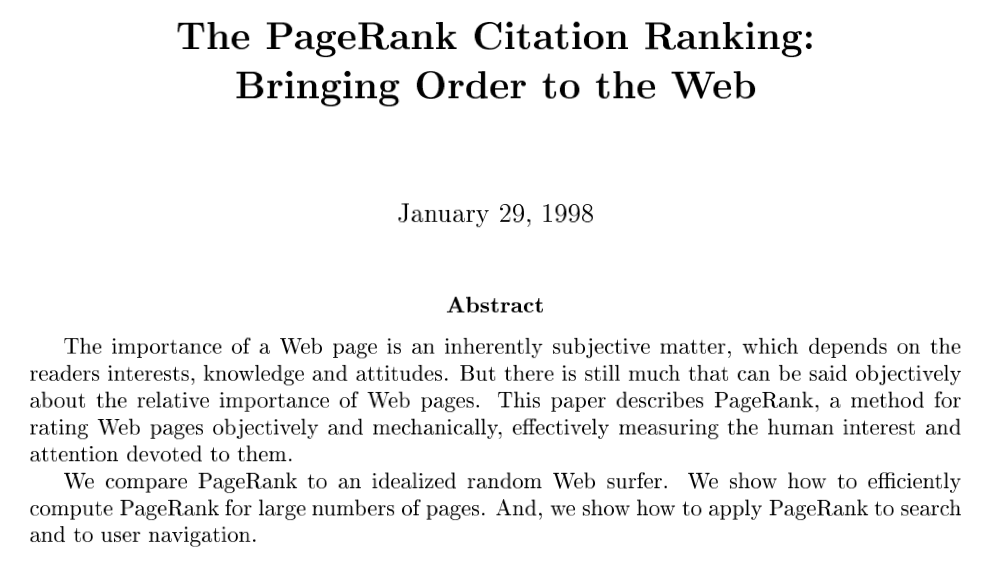
\includegraphics{figs/Aula09/PR-paper.png}

\hypertarget{google}{%
\subsection{Google}\label{google}}

Uma grande inovação do final dos anos 90 é o surgimento das ferramentas
de busca, começando com Alta Vista do DEC's Western Research Lab e tendo
como ápice o Google, fundado pelos doutorandos de Stanford Larry Page e
Sergey Brin

\includegraphics{figs/Aula09/page_brin.webp}

\hypertarget{google-1}{%
\subsection{Google}\label{google-1}}

\begin{tcolorbox}[enhanced jigsaw, colbacktitle=quarto-callout-note-color!10!white, colframe=quarto-callout-note-color-frame, opacityback=0, breakable, toprule=.15mm, leftrule=.75mm, titlerule=0mm, coltitle=black, bottomtitle=1mm, colback=white, toptitle=1mm, title=\textcolor{quarto-callout-note-color}{\faInfo}\hspace{0.5em}{Note}, arc=.35mm, rightrule=.15mm, bottomrule=.15mm, left=2mm, opacitybacktitle=0.6]
O coração da ferramenta de busca do Google é o algoritmo PageRank,
escrito por Larry Page, Sergey Brin, Rajeev Motwani (que se afogou em
acidente trágico em 2009) e Terry Winograd.
\end{tcolorbox}

\hypertarget{fundamentos-do-pagerank}{%
\subsection{Fundamentos do PageRank}\label{fundamentos-do-pagerank}}

\begin{itemize}
\item
  Tipicamente uma ferramenta de busca encontra centenas ou milhares de
  respostas relevantes a uma consulta
\item
  \textbf{Problema:} como ordenar as respostas recuperadas?
\end{itemize}

\hypertarget{possuxedveis-soluuxe7uxf5es}{%
\subsection{Possíveis soluções}\label{possuxedveis-soluuxe7uxf5es}}

Usar a frequência com que os termos buscados aparecem na página Analisar
o histórico de acesso às páginas, para definir as mais importantes

\begin{tcolorbox}[enhanced jigsaw, colbacktitle=quarto-callout-important-color!10!white, colframe=quarto-callout-important-color-frame, opacityback=0, breakable, toprule=.15mm, leftrule=.75mm, titlerule=0mm, coltitle=black, bottomtitle=1mm, colback=white, toptitle=1mm, title=\textcolor{quarto-callout-important-color}{\faExclamation}\hspace{0.5em}{Important}, arc=.35mm, rightrule=.15mm, bottomrule=.15mm, left=2mm, opacitybacktitle=0.6]
Estas soluções não são muito objetivas, nem escaláveis!
\end{tcolorbox}

\hypertarget{section-1}{%
\subsection{}\label{section-1}}

\begin{tcolorbox}[enhanced jigsaw, colbacktitle=quarto-callout-tip-color!10!white, colframe=quarto-callout-tip-color-frame, opacityback=0, breakable, toprule=.15mm, leftrule=.75mm, titlerule=0mm, coltitle=black, bottomtitle=1mm, colback=white, toptitle=1mm, title=\textcolor{quarto-callout-tip-color}{\faLightbulb}\hspace{0.5em}{Tip}, arc=.35mm, rightrule=.15mm, bottomrule=.15mm, left=2mm, opacitybacktitle=0.6]
Felizmente, existe uma estrutura subjacente que pode ser usada para
resolver ambos os problemas: os links entre as páginas!
\end{tcolorbox}

\hypertarget{ideia-original-do-google}{%
\subsection{Ideia original do Google}\label{ideia-original-do-google}}

\begin{itemize}
\tightlist
\item
  Pagerank (importância) de uma página i é baseada nos links que recebe
  de outras páginas:

  \begin{itemize}
  \tightlist
  \item
    Se i recebe links de páginas com pagerank alto, links contribuem
    bastante (recursão!)
  \item
    Se as páginas que tem link para i, tem link para muitas páginas,
    contribuição é menor
  \end{itemize}
\end{itemize}

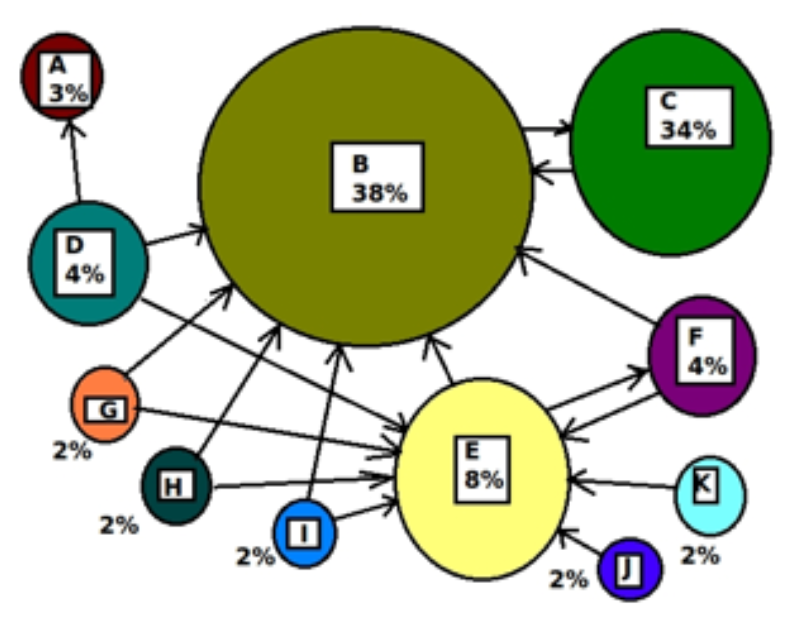
\includegraphics{figs/Aula09/ideia.png}

\hypertarget{brokenrank-quase-pagerank}{%
\subsection{\texorpdfstring{\emph{BrokenRank} (quase
PageRank)}{BrokenRank (quase PageRank)}}\label{brokenrank-quase-pagerank}}

Seja \(L_{ij} = 1\) se a página \(j\) tem \emph{link} para a página
\(i\) (\(j\rightarrow i\)) e \(L{ij} = 0\) caso contrário. Sejam
\(m_j=\sum_k L_{kj}\) o grau de saída de \(j\). O \emph{BrokenRank}
\(p_i\) da página \(i\) será

\[ p_i = \sum_{j\rightarrow i} \frac{p_j}{m_j} = \sum_{j=1}^n \frac{L_{ij}}{m_j}p_j \]

\begin{tcolorbox}[enhanced jigsaw, colbacktitle=quarto-callout-caution-color!10!white, colframe=quarto-callout-caution-color-frame, opacityback=0, breakable, toprule=.15mm, leftrule=.75mm, titlerule=0mm, coltitle=black, bottomtitle=1mm, colback=white, toptitle=1mm, title=\textcolor{quarto-callout-caution-color}{\faFire}\hspace{0.5em}{Danger}, arc=.35mm, rightrule=.15mm, bottomrule=.15mm, left=2mm, opacitybacktitle=0.6]
Essa definição satisfaz as condições anteriores?
\end{tcolorbox}

\hypertarget{brokenrank-em-notauxe7uxe3o-matricial}{%
\subsection{\texorpdfstring{\emph{BrokenRank} em notação
matricial}{BrokenRank em notação matricial}}\label{brokenrank-em-notauxe7uxe3o-matricial}}

\[p = \begin{bmatrix}p_1 \\ p_2\\ \vdots \\ p_n\end{bmatrix}_{n\times 1}, L = \begin{bmatrix}L_{11} & L_{12} & \ldots & L_{1n}\\ L_{21} & L_{22} & \ldots & L_{2n} \\ \vdots &\vdots&\ddots&\vdots\\ L_{n1} & L_{n2} & \ldots & L_{nn}\end{bmatrix}_{n\times n}\]

\[M = \begin{bmatrix}m_1 & 0 &\ldots & 0\\ 0 & m_2 & \ldots & 0\\\vdots &\vdots&\ddots&\vdots\\ 0 & 0 & \dots & m_n\end{bmatrix}_{n\times n}\]

Vetor \emph{BrokenRank} de \(p\)

\[ p = LM^{-1}p\]

\hypertarget{autovalroes-e-autovetores}{%
\subsection{Autovalroes e Autovetores}\label{autovalroes-e-autovetores}}

Seja \(A = LM^{-1}\), então \(p = Ap\). O que isso quer dizer?

\begin{tcolorbox}[enhanced jigsaw, colbacktitle=quarto-callout-important-color!10!white, colframe=quarto-callout-important-color-frame, opacityback=0, breakable, toprule=.15mm, leftrule=.75mm, titlerule=0mm, coltitle=black, bottomtitle=1mm, colback=white, toptitle=1mm, title=\textcolor{quarto-callout-important-color}{\faExclamation}\hspace{0.5em}{Important}, arc=.35mm, rightrule=.15mm, bottomrule=.15mm, left=2mm, opacitybacktitle=0.6]
p é um \textbf{autovetor} de \(A\) com \textbf{autovalor} 1!
\end{tcolorbox}

Agora precisamos saber como calcular os \textbf{autovalores} e
\textbf{autovetores} de \(A\). Existem métodos eficientes para isso
quando \(A\) é \textbf{grande e esparsa}. Por que isso se aplica nesse
caso?

\hypertarget{random-surfer-model}{%
\subsection{\texorpdfstring{\emph{Random Surfer}
model}{Random Surfer model}}\label{random-surfer-model}}

Podemos pensar no BrokenRank como um usuário que surfa a Web clicando
nos links de maneira uniformemente aleatória

Suponha que \(p^{(0)}\) seja o vetor n-dimensional que dá a
probabilidade de começar em cada página. Depois de um passo, a
probabilidade de estar em cada página é dada por \(p^{(1)} = Ap^{(0)}\).
(Por quê?)

\[p^{(1)} = p_1^{(0)}\frac{L_{i1}}{m_1} +  p_2^{(0)}\frac{L_{i2}}{m_2} + \ldots + p_n^{(0)}\frac{L_{in}}{m_n} = \sum_{i=1}^n\frac{L_{ij}}{mij}p_j^{(0)}\]

\[p^{(i+1)} = A p^{(i)}\]

\hypertarget{conexuxe3o-c-cadeias-de-markov}{%
\subsection{Conexão c/ cadeias de
Markov}\label{conexuxe3o-c-cadeias-de-markov}}

\begin{itemize}
\item
  A matriz \(A\) é uma matriz de transição de probabilidade que governa
  uma Cadeia de Markov.
\item
  Teoria de Cadeias de Markov nos diz que o vetor \(p^{(t)}\) converge
  para um \(p\) único quando o grafo é:

  \begin{itemize}
  \tightlist
  \item
    Fortemente conectado (cada página possui caminho p/ todas outras
    páginas) e
  \item
    É não-bipartido
  \item
    Não periódico
  \end{itemize}
\end{itemize}

\textbf{Interpretação:} \(p_i\) é a proporção do tempo que o usuário
passa na página \(i\) se deixarmos ele navegar infinitamente.

\hypertarget{por-que-brokenrank-uxe9-broken}{%
\subsection{\texorpdfstring{Por que \emph{BrokenRank} é
\emph{broken}?}{Por que BrokenRank é broken?}}\label{por-que-brokenrank-uxe9-broken}}

Problema: o grafo sobre o qual o \emph{random surfer} navega não é
fortemente conectado 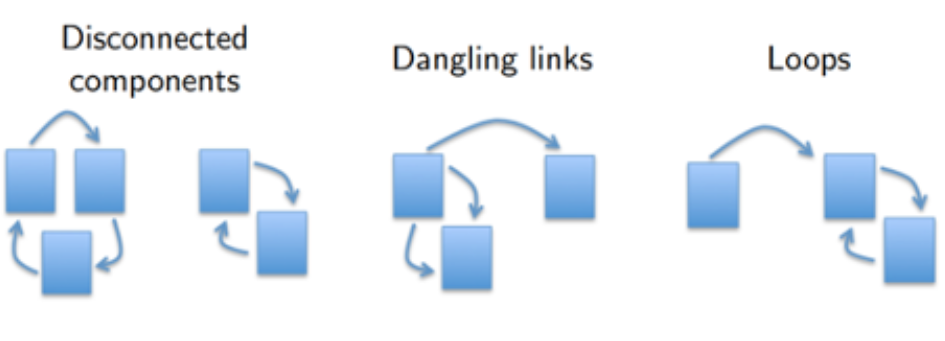
\includegraphics{figs/Aula09/PR_componentes.png}

\begin{tcolorbox}[enhanced jigsaw, colbacktitle=quarto-callout-note-color!10!white, colframe=quarto-callout-note-color-frame, opacityback=0, breakable, toprule=.15mm, leftrule=.75mm, titlerule=0mm, coltitle=black, bottomtitle=1mm, colback=white, toptitle=1mm, title=\textcolor{quarto-callout-note-color}{\faInfo}\hspace{0.5em}{Note}, arc=.35mm, rightrule=.15mm, bottomrule=.15mm, left=2mm, opacitybacktitle=0.6]
Vetor p sempre existe, mas pode não ser único. Ou seja, o vetor
BrokenRank \(p\) existe, mas é ambíguo.
\end{tcolorbox}

\hypertarget{exemplo-com-brokenrank}{%
\subsection{\texorpdfstring{Exemplo com
\emph{BrokenRank}}{Exemplo com BrokenRank}}\label{exemplo-com-brokenrank}}

\[ A = LM^{-1} = \begin{bmatrix}0&0&1&0&0\\1&0&0&0&0\\0&1&0&0&0\\0&0&0&0&1\\0&0&0&1&0\end{bmatrix}\]

\begin{figure}

{\centering 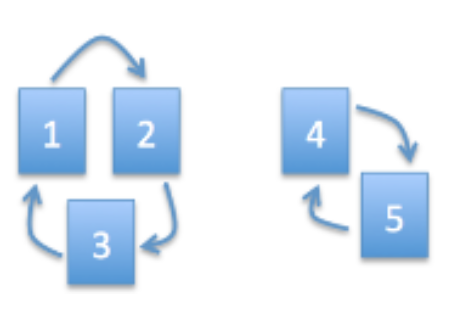
\includegraphics{figs/Aula09/exemplo_BR.png}

}

\caption{Grafo de conectividade}

\end{figure}

2 autovetores de \(A\) com \(\lambda=1\)

\[p = \begin{bmatrix}\frac{1}{3}\\\frac{1}{3}\\\frac{1}{3}\\0\\0\end{bmatrix} \text{ e } \begin{bmatrix}0\\0\\0\\\frac{1}{2}\\\frac{1}{2}\end{bmatrix}\]

\begin{tcolorbox}[enhanced jigsaw, colbacktitle=quarto-callout-important-color!10!white, colframe=quarto-callout-important-color-frame, opacityback=0, breakable, toprule=.15mm, leftrule=.75mm, titlerule=0mm, coltitle=black, bottomtitle=1mm, colback=white, toptitle=1mm, title=\textcolor{quarto-callout-important-color}{\faExclamation}\hspace{0.5em}{Important}, arc=.35mm, rightrule=.15mm, bottomrule=.15mm, left=2mm, opacitybacktitle=0.6]
Estes \emph{rankings} são totalmente opostos!
\end{tcolorbox}

\hypertarget{definiuxe7uxe3o-de-pagerank}{%
\subsection{\texorpdfstring{Definição de
\emph{PageRank}}{Definição de PageRank}}\label{definiuxe7uxe3o-de-pagerank}}

\begin{itemize}
\item
  \emph{PageRank} é uma pequena variação do \emph{BrokenRank}
\item
  Com probabilidade \(1-d\) o random surfer dá um salto aleatório
  (escolhe uma página uniformemente do universo de páginas);
\item
  Com probabilidade \(d\) ele escolhe um dos links da página atual de
  maneira uniforme aleatória.
\end{itemize}

\hypertarget{definiuxe7uxe3o-de-pagerank-1}{%
\subsection{\texorpdfstring{Definição de
\emph{PageRank}}{Definição de PageRank}}\label{definiuxe7uxe3o-de-pagerank-1}}

\begin{itemize}
\tightlist
\item
  \emph{PageRank} é uma pequena variação do \emph{BrokenRank}
\end{itemize}

\[ p_i = \frac{1-d}{n} + d\sum_{j\rightarrow i} \frac{p_j}{m_j} = \frac{1-d}{n} + d\sum_{j=1}\frac{L_{ij}}{m_j}p_j\]

onde \(0<d<1\) é uma constante (ex: \(d=0.85\))

Em notação matricial

\[ p =  \left( \frac{1-d}{n}E + dLM^{-1}\right)p\]

onde \(E\) é a matriz \(n\times n\) de \(1s\)

\hypertarget{definiuxe7uxe3o-do-pagerank}{%
\subsection{\texorpdfstring{Definição do
\emph{PageRank}}{Definição do PageRank}}\label{definiuxe7uxe3o-do-pagerank}}

Conferindo equivalência das duas definições

\[ p_i = \frac{1-d}{n} + d\sum_{j\rightarrow i} \frac{p_j}{m_j} = \frac{1-d}{n} + d\sum_{j=1}\frac{L_{ij}}{m_j}p_j\]

\[ p = \left(\frac{1-d}{n}E + dLM^{-1}\right)p\]

\[ \begin{bmatrix}p\end{bmatrix} = \frac{1-d}{n}\begin{bmatrix}1&\ldots&1\\\vdots&\ddots&\vdots\\1&\ldots&1\end{bmatrix}\begin{bmatrix}p\end{bmatrix} + d\begin{bmatrix}LM^{-1}\end{bmatrix}\begin{bmatrix}p\end{bmatrix}\]

\[ \begin{bmatrix}p\end{bmatrix} = 1-d\begin{bmatrix}1/n&\ldots&1/n\\\vdots&\ddots&\vdots\\1/n&\ldots&1/n\end{bmatrix}\begin{bmatrix}p\end{bmatrix} + d\begin{bmatrix}LM^{-1}\end{bmatrix}\begin{bmatrix}p\end{bmatrix}\]

\[p_i = \frac{1-d}{n}(p_1+p_2+\dots+p_n) + d \sum_{i=1}^n \frac{L_{ij}}{m_j}p_j\]

\[p_i = \frac{1-d}{n} + d \sum_{i=1}^n \frac{L_{ij}}{m_j}p_j\]

\hypertarget{pagerank-possui-p-uxfanico}{%
\subsection{\texorpdfstring{\emph{PageRank} possui \(p\)
único}{PageRank possui p único}}\label{pagerank-possui-p-uxfanico}}

Este modelo é um \emph{random surfer} com \emph{random jumps}

Agora existe um caminho de cada página para todas as outras páginas.
Portanto, o vetor \(p\) é único (quando sujeito à restrição
\(\sum_{i} p_i = 1\)).


\includegraphics{figs/Aula09/randomSurfer.png}

\hypertarget{exemplo}{%
\subsection{Exemplo}\label{exemplo}}

Com \(d = 0.85, A= \frac{1-d}{n}E + d LM^{-1}\)

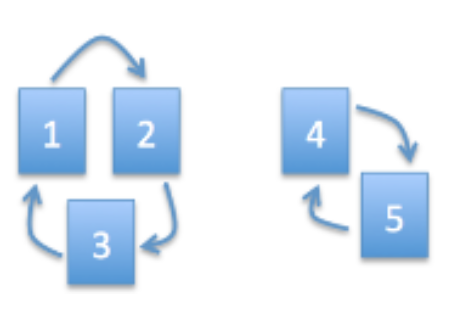
\includegraphics{figs/Aula09/exemplo_BR.png}

\hypertarget{exemplo-1}{%
\subsection{Exemplo}\label{exemplo-1}}

Com \(d = 0.85, A= \frac{1-d}{n}E + d LM^{-1}\)

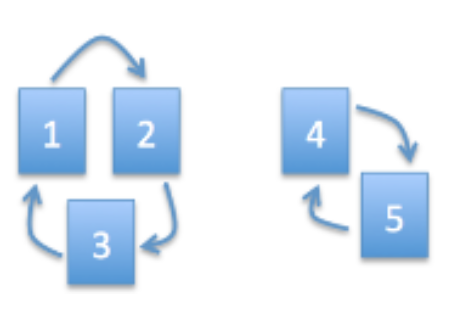
\includegraphics{figs/Aula09/exemplo_BR.png}

\begin{align}
&= \frac{0.15}{5}\begin{bmatrix}1 & 1 & 1 & 1 & 1\\1 & 1 & 1 & 1 & 1\\1 & 1 & 1 & 1 & 1\\1 & 1 & 1 & 1 & 1\\1 & 1 & 1 & 1 & 1\end{bmatrix} + 0.85\begin{bmatrix}0 & 0 & 1 & 0 & 0\\1 & 0 & 0 & 0 & 0\\0 & 1 & 0 & 0 & 0\\0 & 0 & 0 & 0 & 1\\0 & 0 & 0 & 1 & 0\end{bmatrix}\\

&= \begin{bmatrix}0.03 & 0.03 & 0.88 & 0.03 & 0.03\\0.88 & 0.03 & 0.03 & 0.03 & 0.03\\0.03 & 0.88 & 0.03 & 0.03 & 0.03\\0.03 & 0.03 & 0.03 & 0.03 & 0.88\\0.03 & 0.03 & 0.03 & 0.88 & 0.03\end{bmatrix}
\end{align}

Agora possui apenas um autovetor

\[ p = \begin{bmatrix}0.2\\0.2\\0.2\\0.2\\0.2\end{bmatrix}\]

\hypertarget{computando-o-vetor-pagerank}{%
\subsection{\texorpdfstring{Computando o vetor
\emph{PageRank}}{Computando o vetor PageRank}}\label{computando-o-vetor-pagerank}}

\begin{itemize}
\item
  Poderíamos calcular o vetor \emph{PageRank} \(p\) com decomposição
  espectral, mas o custo é da ordem de \(n^3\) operações. Quando
  \(n=3\times 10^{10}\), \(n^3 = 2.7x10^{31}…\) (isto sem falar na
  memória)
\item
  Felizmente, só precisamos do autovetor com \(\lambda=1\). Melhor
  ainda: sabe-se que todos os outros autovalores tem valor absoluto
  \(< 1\).
\end{itemize}

\hypertarget{computando-o-vetor-pagerank-1}{%
\subsection{\texorpdfstring{Computando o vetor
\emph{PageRank}}{Computando o vetor PageRank}}\label{computando-o-vetor-pagerank-1}}

Lembrando que

\[ p^{(i)} = A p^{(i-1)}= A^2p^{(i-2)} = A^3p^{(i-3)}\ldots\]

\[p = c_1x_1 + c_2x_2 + \ldots + c_nx_n\]

\[A^kp = c_1\lambda^k x_1 + \ldots + c_n\lambda_n^kx_n\]

Sem perda de generalidade, suponha

\[ \lambda_1 = 1 > \vert \lambda_2\vert \ge \vert \lambda_3 \vert \ge \ldots \ge \vert \lambda_n\vert\]

O que acontece se pré-multiplicarmos o vetor \(p^{(0)}\) por \(A\)
muitas vezes?

\textbf{Resposta}: quando \(t\rightarrow \infty\) vai convergir para
\(c_1x_1\)

\begin{tcolorbox}[enhanced jigsaw, colbacktitle=quarto-callout-note-color!10!white, colframe=quarto-callout-note-color-frame, opacityback=0, breakable, toprule=.15mm, leftrule=.75mm, titlerule=0mm, coltitle=black, bottomtitle=1mm, colback=white, toptitle=1mm, title=\textcolor{quarto-callout-note-color}{\faInfo}\hspace{0.5em}{Note}, arc=.35mm, rightrule=.15mm, bottomrule=.15mm, left=2mm, opacitybacktitle=0.6]
Lembrando que \(c_1x_1\) é uma constante vezes o autovetor cujo
autovalor é igual a 1
\end{tcolorbox}

\hypertarget{muxe9todo-da-potuxeancia-power-method}{%
\subsection{Método da potência (Power
Method)}\label{muxe9todo-da-potuxeancia-power-method}}

Comece com qualquer distribuição \(p^{(0)}\) (ex: uniforme)

Faça:

\begin{align}
p^{(1)} &= Ap^{(0)}\\
p^{(2)} &= Ap^{(1)}\\
\vdots\\
p^{(t)} &= Ap^{(t-1)}\approx c_1x_1\\
\end{align}

\begin{tcolorbox}[enhanced jigsaw, colbacktitle=quarto-callout-note-color!10!white, colframe=quarto-callout-note-color-frame, opacityback=0, breakable, toprule=.15mm, leftrule=.75mm, titlerule=0mm, coltitle=black, bottomtitle=1mm, colback=white, toptitle=1mm, title=\textcolor{quarto-callout-note-color}{\faInfo}\hspace{0.5em}{Note}, arc=.35mm, rightrule=.15mm, bottomrule=.15mm, left=2mm, opacitybacktitle=0.6]
Não precisamos nos preocupar com \(c_1\), pois basta normalizar (soma
um). Na prática normalizamos a cada passo e repetimos até que \(p\) não
mude ``muito''
\end{tcolorbox}

\hypertarget{muxe9todo-da-potuxeancia-exemplo}{%
\subsection{Método da potência
(Exemplo)}\label{muxe9todo-da-potuxeancia-exemplo}}

Comece com qualquer distribuição (ex: uniforme)
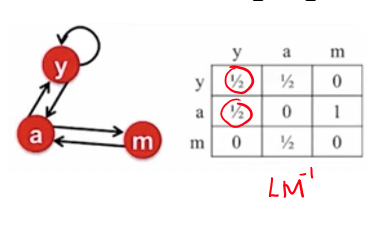
\includegraphics[width=0.6\textwidth,height=\textheight]{figs/Aula09/ex_metodo_potencia.png}

\[ p^{(0)} = \begin{bmatrix}1/3\\1/3\\1/3\end{bmatrix}\]

\begin{align}
A &= \frac{1-d}{n}E + dLM^{-1}\\
&= \begin{bmatrix}0.05 & 0.05 & 0.05\\0.05 &0.05&0.05\\0.05&0.05&0.05\end{bmatrix} + \begin{bmatrix}0.425 & 0.425&0\\0.425&0&0.85\\0&0.425&0\end{bmatrix}\\
p^{(1)} &= \begin{bmatrix}0.475&0.475&0.05\\0.475&0.05&0.9\\0.05&0.475&0.05\end{bmatrix}\begin{bmatrix}1/3\\1/3\\1/3\end{bmatrix}\\
p^{(1)}&= \begin{bmatrix}0.333\\0.475\\0.192\end{bmatrix}\\
p^{(2)} &= \begin{bmatrix}0.475&0.475&0.05\\0.475&0.05&0.9\\0.05&0.475&0.05\end{bmatrix}\begin{bmatrix}0.333\\0.495\\0.192\end{bmatrix}\\
p^{(2)}&= \begin{bmatrix}0.394\\0.355\\0.252\end{bmatrix}
\end{align}

\hypertarget{muxe9todo-da-potuxeancia-continuauxe7uxe3o}{%
\subsection{Método da potência
(continuação)}\label{muxe9todo-da-potuxeancia-continuauxe7uxe3o}}

\begin{itemize}
\tightlist
\item
  Há ainda duas questões importantes sobre o cálculo do vetor pagerank
  \(p\) usando power method

  \begin{itemize}
  \tightlist
  \item
    Como executar cada iteração rapidamente? (custo de multiplicar
    matriz por vetor é \(O(n^2)\)).
  \item
    Quantas iterações \(t\) são necessárias?
  \end{itemize}
\end{itemize}

\hypertarget{muxe9todo-da-potuxeancia-continuauxe7uxe3o-1}{%
\subsection{Método da potência
(continuação)}\label{muxe9todo-da-potuxeancia-continuauxe7uxe3o-1}}

\begin{itemize}
\tightlist
\item
  A grosso modo, as respostas são:

  \begin{itemize}
  \tightlist
  \item
    Usando a esparsidade do grafo da web (como?)
  \item
    Não muitas se o spectral gap (diferença entre primeiro e segundo
    maiores autovalores absolutos) for grande; o maior é 1, o segundo
    maior é \(\le d\).
  \end{itemize}
\end{itemize}

\hypertarget{uma-busca-buxe1sica-na-web}{%
\subsection{Uma busca básica na Web}\label{uma-busca-buxe1sica-na-web}}

Solução 1: Para fazer uma busca na web e responder uma consulta, podemos

\begin{enumerate}
\def\labelenumi{\arabic{enumi}.}
\tightlist
\item
  Calcular o vetor \emph{PageRank} \(p\) uma vez (Google recomputa-o de
  tempos em tempos).
\item
  Encontre os documentos contendo todas palavras da consulta.
\item
  Ordene estes documentos por \emph{PageRank} e retorne os top \(k\)
  (e.g.~\(k=50\))
\end{enumerate}

\hypertarget{uma-busca-buxe1sica-na-web-1}{%
\subsection{Uma busca básica na
Web}\label{uma-busca-buxe1sica-na-web-1}}

Podemos melhorar solução usando escores de similaridade entre página e
consulta.

Solução 2: (passos 1 e 2 iguais à anterior)

\begin{enumerate}
\def\labelenumi{\arabic{enumi}.}
\setcounter{enumi}{2}
\tightlist
\item
  Ordene estes documentos por PageRank e mantenha apenas os top K
  (e.g.~\(K=5000\))
\item
  Ordene por similaridade à consulta (e.g., normalized IDF
  weighted-distance), e retorne os top k (e.g., \(k=50\))
\end{enumerate}

\hypertarget{variantes-extensuxf5es-do-pagerank}{%
\subsection{\texorpdfstring{Variantes / Extensões do
\emph{PageRank}}{Variantes / Extensões do PageRank}}\label{variantes-extensuxf5es-do-pagerank}}

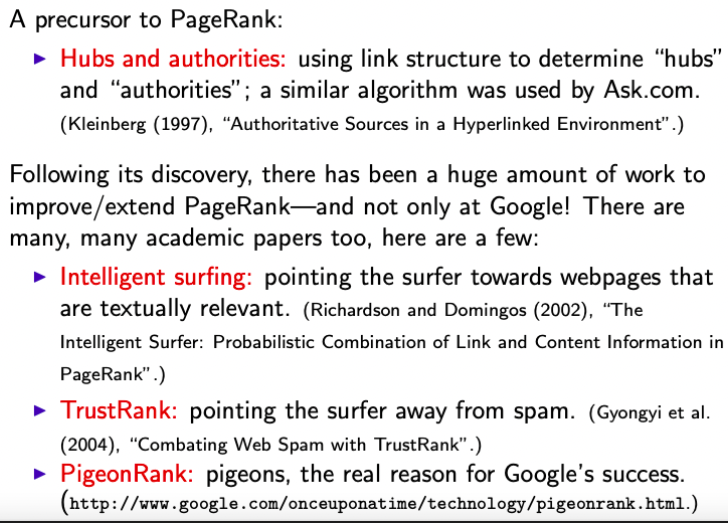
\includegraphics{figs/Aula09/variantes.png}



\end{document}
